\begin{frame}[fragile]{Tutorial: One-site operators}

\begin{columns}

\begin{column}{4.5cm}

\begin{onlyenv}<1->
\begin{lstlisting}[language=JuliaLocal, style=julia, basicstyle=\scriptsize\ttfamily]
Z = op("Z", i)
X = op("X", i)

Zp = state("Zp", i)
Zm = state("Zm", i)
\end{lstlisting}
\end{onlyenv}

\begin{onlyenv}<3->
\begin{lstlisting}[language=JuliaLocal, style=julia, basicstyle=\scriptsize\ttfamily]
X * Zp == Zm'
noprime(X * Zp) == Zm
\end{lstlisting}
\end{onlyenv}

\end{column}

\begin{column}{4.5cm}

\begin{onlyenv}<1-1>
Z \\
X \\
~\\
|Z+$\rangle$ \\
|Z-$\rangle$ \\
\end{onlyenv}

\begin{onlyenv}<2->
\begin{center}
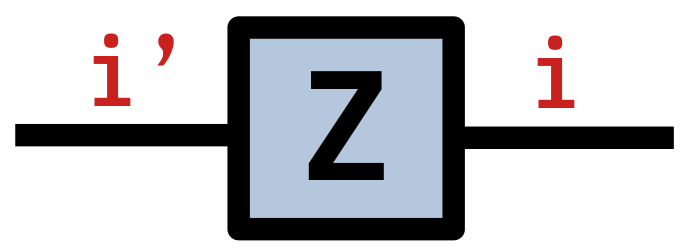
\includegraphics[width=0.45\textwidth]{
  slides/assets/Z.png
} \
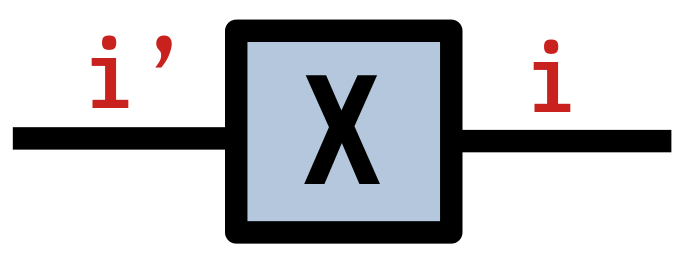
\includegraphics[width=0.45\textwidth]{
  slides/assets/X.png
} \\
\vspace*{0.5cm}
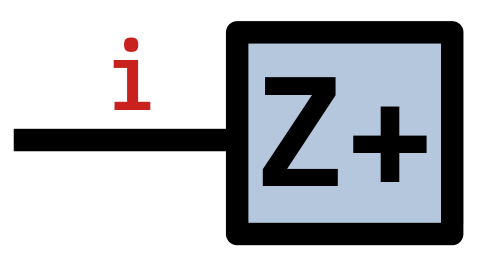
\includegraphics[width=0.35\textwidth]{
  slides/assets/Zp.png
} \ \ \ \ 

\includegraphics[width=0.35\textwidth]{
  slides/assets/Zm.png
}
\end{center}
\vspace*{0.1cm}
\end{onlyenv}

\begin{onlyenv}<3-3>
~\\
X|Z+$\rangle$ = |Z-$\rangle$ \\
~\\
~\\
~\\
\end{onlyenv}

\begin{onlyenv}<4->
\vspace*{0.3cm}
\begin{center}

\includegraphics[width=1.0\textwidth]{
  slides/assets/XZp.png
}
\end{center}
\vspace*{0.2cm}
\end{onlyenv}

\end{column}

\end{columns}

\end{frame}
